\documentclass[11pt, a4paper]{book}
\errorcontextlines 10000
\usepackage[utf8]{inputenc}
\usepackage[italian]{babel}
\usepackage[T1]{fontenc}

\usepackage{tabularx}
\usepackage[table]{xcolor}

% required to include the thesis first page
\usepackage{pdfpages}

% specifying lmodern as default font, uses it on the entire document
% (before doing this, It used different fonts along the document...)
\usepackage{lmodern}

% listing required for quote management
\usepackage{textcomp}

\usepackage{graphicx}
\usepackage{wrapfig}
\graphicspath{ {immagini/} }

\usepackage{mathtools}

\usepackage{listings}
\renewcommand{\lstlistingname}{Listato}
\renewcommand{\lstlistlistingname}{Elenco dei listati}
\lstset{upquote=true, breaklines=true, columns=flexible}
% Thanks to: https://tex.stackexchange.com/questions/64839/how-to-change-listing-caption

\usepackage[backend=biber]{biblatex}
\addbibresource{thesis_citations.bib}

\usepackage[justification=justified]{caption}
\usepackage{subcaption}

\usepackage[binary-units=true]{siunitx}

%TODO: source https://tex.stackexchange.com/questions/9796/how-to-add-todo-notes
\usepackage[colorinlistoftodos,prependcaption,textsize=tiny]{todonotes}

\newcommand{\addcontent}[1]{\todo[inline,linecolor=green,backgroundcolor=green!25,bordercolor=green,]{#1}}

\newcommand {\pygfa} {\textit{PyGFA }}

\title{\pygfa \\
	Progettazione ed implementazione di una libreria Python per la gestione
	di file GFA}
\author{Diego Lobba}

\begin{document}
% \maketitle
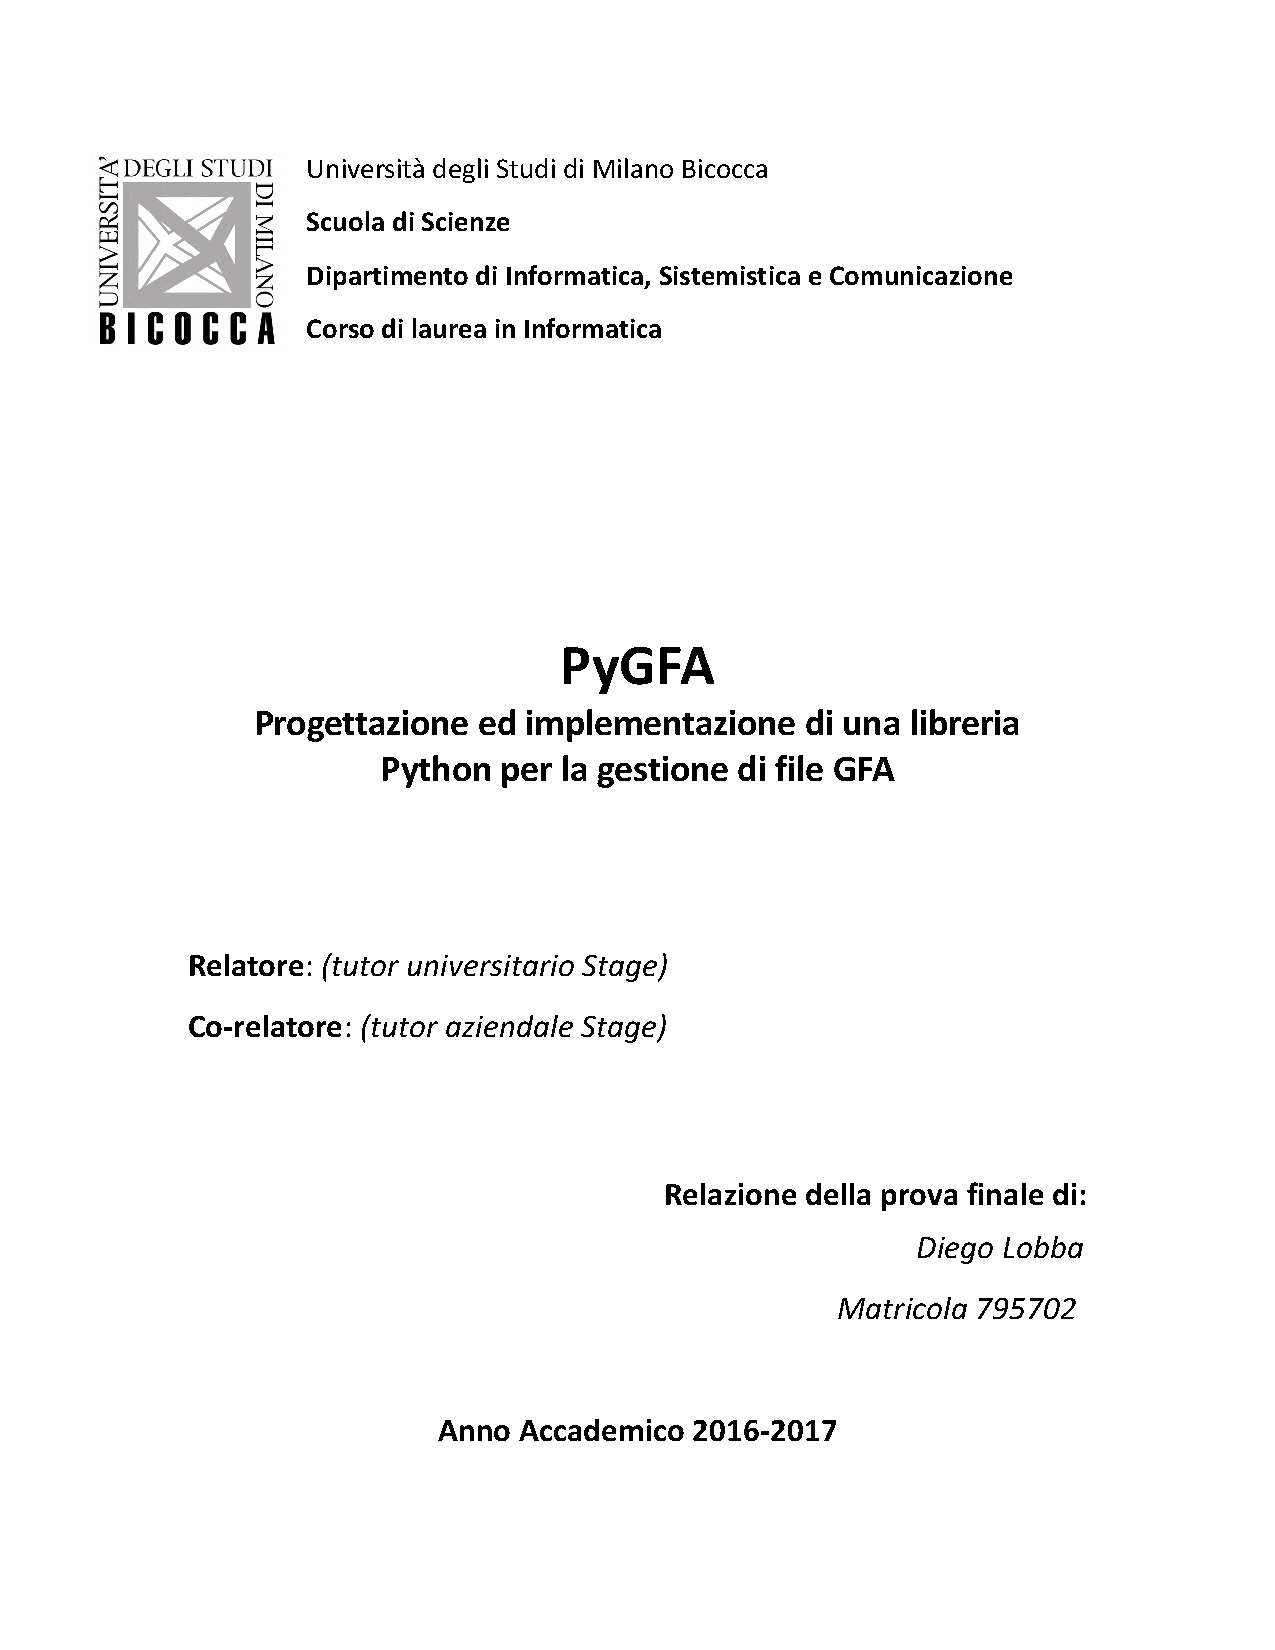
\includepdf[pages={1}]{immagini/frontespiziorelazionefinale20162017.pdf}

\tableofcontents
\listoffigures

\chapter{Panoramica su \pygfa}
\pygfa è una libreria Python che permette di gestire le informazioni
contenute in file GFA rappresentandole mediante una struttura a grafo.
La gestione delle operazioni sul grafo avviene sfruttando una libreria
preesistente: \emph{networkx}\cite{networkx}, per la quale \pygfa si occupa di fornire
le interfacce ai metodi.

\pygfa inoltre permette l'attraversamento del grafo mediante interatori
personalizzati, che considerano solamente archi rappresentanti un
determinato tipo di connessione (\emph{dovetail overlap}) fra i nodi del
grafo.

I file GFA\cite{gfa_spec} (Graphical Fragment Assembly) sono file che descrivono	
i legami fra sequenze genomiche di un organismo. Ogni sequenza
viene vista come un nodo sul quale possono esserci collegate altre
sequenze per mezzo di collegamenti. Tali collegamenti possono
coinvolgere la sequenza secondo due direzioni:
\begin{itemize}
	\item la prima, indicata dal simbolo \textbf{+}, considera la
	sequenza così come appare nella sua definizione all'interno del file,
	\item la seconda, indicata dal simbolo \textbf{-}, considera la
	sequenza dopo che su di essa viene effettuata un'operazione di
	\emph{reverse and complement}.
\end{itemize}

I file GFA possono arrivare a contenere milioni tra sequenze e collegamenti
presenti tra di loro, per questo motivo si è voluto sviluppare una libreria
in grado di gestire tali file permettendo non solo di andare ad effettuare
operazioni di filtraggio e selezione sulle informazioni contenute, ma
anche in grado di fornire una serie di strumenti per la loro
manipolazione ed ulteriore analisi.

\section{RGFA e GfaPy}
\pygfa non è la sola libreria che gestisce file GFA mediante una struttura a grafo.
RGFA è una libreria scritta in Ruby creata appositamente per questo scopo e GfaPy
è l'equivalente riscritta in Python. GfaPy non solo implementa le funzionalità di RGFA,
ma estende il supporto alla specifica GFA2 (che verrà successivamente illustrata).

Nonostante le somiglianze fra GfaPy e \pygfa, le due librerie non solo differiscono
a livello implementativo, ma hanno una gestione dei dati completamente diversa.
Le informazioni in GfaPy continuano a tenere informazioni sulla loro origine (il tipo
di linea dalla quale provengono). In \pygfa invece le informazioni vengono	
ricondotte ad un unico livello di astrazione; tutti i collegamenti possiedono tutti
lo stesso numero di campi, i quali seccessivamente potranno averli definiti o meno
a seconda del tipo di linea/collegamento. Questo approccio di \pygfa è stato
preferito per tenere una coerenza generale nei dati usati dal grafo networkx
sottostante e per avere un'informazione che l'utente della libreria può interpretare
in senso più ampio; slegato dal concetto che la specifica GFA le assegna, ma
rappresentante il concetto biologico che tale informazione vuole significare.

\chapter{Ecosistema e strumenti}
\label{ch:ecosistema}
In questo capitolo verranno descritti i linguaggi utilizzati e gli
strumenti impiegati nell'analisi, nello sviluppo e nei test della libreria.
Di ogni elemento verrà fornita una breve panoramica, ponendo
maggior enfasi sugli aspetti (alle volte piuttosto tecnici) che è
stato necessario tenere in considerazione durante lo sviluppo
di \pygfa.

\section{Il linguaggio Python}
\nocite{wiki-python}
Python è un linguaggio di programmazione ideato da Guido van Rossum
all'inizio degli anni `90. Python è un linguaggio che si appresta a molteplici
stili di programmazione, sfruttando caratteristiche del paradigma object
oriented, funzionale e della programmazione strutturata.
Tali proprietà permetto l'uso del linguaggio in una grande varietà di attività:
nella creazione di script di automazione di sistema, nella scrittura di
sistemi web di backend fino allo sviluppo di complesse librerie di analisi numerica
e machine learning.

\begin{wrapfigure} {O} {0.35\textwidth}
	\begin{centering}	
		
\includegraphics{python-logo}
		\caption[Logo Python]{Logo del linguaggio di programmazione Python.}
	\end{centering}
\end{wrapfigure}
La minima struttura necessaria a produrre un programma Python,
l'inferenza del tipo delle variabili a runtime (\emph{dynamic typing}),
la gestione automatica della memoria e la sua espressività lo rendono
un candidato ideale nella prototipazione di sistemi nuovi, coerente con
processi di sviluppo agili e con la pratica di extreme programming.

Inoltre Python è un linguaggio interpretato, di conseguenza è possibile
effettuare, direttamente all'interno dell'interprete, verifiche in tempo
reale delle funzionalità attualmente in sviluppo.
Il fatto che il linguaggio venga interpretato
da un interprete permette una facile integrazione del codice nativo
con il quale l'interprete stesso è stato implementato.
Per questo motivo -e grazie al livello di astrazione sul quale si colloca-
esistono diverse implementazioni del linguaggio Python
che sfruttano la JVM, la piattaforma .NET, il linguaggio C o che si
concentrano maggiormente su alcuni aspetti specifici come la velocità,
il multithreading e la minimalità per l'uso in ambienti embedded.

\captionsetup{justification=centering, singlelinecheck=false}
\begin{lstlisting}[language=Python, frame=topline, caption=Un esempio  dell'espressività\\del linguaggio applicata a \pygfa.]
>>> import pygfa
>>> gfa = pygfa.gfa.GFA.from_file("data/sample1.gfa")
>>> gfa.nodes()
['1', '3', '2', '5', '13', '6', '11', '12', '4']
>>> pygfa.nodes_connected_components(gfa) #calcola i nodi
	di ciascuna componente connessa
...
[{'2', '1', '3', '6', '5'}, {'11', '13', '12'}, {'4'}]
>>> # estrai tutte le componenti connesse
	con numero di nodi maggiore di 3
...
>>> [component for component in pygfa.nodes_connected_components(gfa)
	if len(component) > 3]
[{'2', '1', '3', '6', '5'}]
\end{lstlisting}
\captionsetup{justification=justified, singlelinecheck=false}

\subsection{Classi, convenzioni e duck typing}
In Python per creare una classe è necessario definirla mediante
la dicitura:
\begin{lstlisting}[language=Python]
class MiaClasse(Antenata1, Antenata2, ...):
	...
\end{lstlisting}
Come è possibile notare, è ammissibile ereditare da più classi.
Tale caratteristica non è molto frequente negli altri linguaggi e
viene spesso considerata una cattiva pratica, visto che non
permette di accorgersi di una errata definizione della gerarchia delle
classi di progetto. Tuttavia, in Python questa proprietà permette
l'aggiunta di funzionalità alla classe, in modo analogo alla modalità
\texttt{implements} di Java, rendendo possibile una definizione di
quelle che in realtà sono le interfacce e le loro implementazioni.
In \pygfa tale funzionalità è stata applicata per aggiungere le
funzionalità degli iteratori personalizzati alla classe \texttt{GFA}.

Python è un linguaggio fortemente influenzato dai movimenti
open source; infatti ogni programma, libreria e sistema scritto in Python
presuppone che l'utilizzatore abbia libero accesso al sorgente e che
possa capire le modalità di utilizzo di ogni modulo di cui è composto.
Per questo motivo i programmi tendono ad essere ricchi di documentazione,
sia essa incorporata nel codice che allegata nel manuale.
Come conseguenza il linguaggio non offre un meccanismo per definire i
metodi di una classe come privati; in virtù del fatto che l'utilizzatore, avendo
la piena possibilità di capire il funzionamento del singlo modulo di sistema,
ha la piena responsabilità delle sue azioni.
Per aiutare a distinguere elementi del programma che l'autore vorrebbe
fossero non utilizzati (o utilizzati con particolare consapevolezza) si è
soliti nominare tali elementi facendo precedere i loro nomi da un singolo
trattino basso (\emph{weak internal use}). E' possibile imprimere
maggior enfasi nell'oscuramento di un elemento precedendo
il suo nome da due trattini bassi, in tal modo l'accesso
all'elemento avviene precendo il nome della classe al nome dell'elemento.

\captionsetup{justification=centering}
\begin{lstlisting}[language=Python, frame=topline, caption=Convenzioni per l'uso interno.]
>>> class A:
...	def __init__(self):
...		self.normal_use = 5
...		self._internal_use = 10
...		self.__strong_internal = 15
...
>>> a = A()
>>> a.normal_use
5
>>> a._internal_use
10
>>> a._A__strong_internal
15
\end{lstlisting}
\captionsetup{justification=justified}

Una ulteriore convenzione comune al Python e ampiamente considerata
nello sviluppo di \pygfa è il cosiddetto \emph{duck typing}.
Visto che il Python usa il binding dinamico, le funzioni e i metodi non
possono verificare il tipo dei parametri passati tramite signature.
Una possibile soluzione è verificare il tipo del parametro mediante
la funzione \texttt{isinstance}, come avviene per esempio quando
si cerca di effettuare il \emph{downcast} dalla classe antenata
ad una sottoclasse nei linguaggi in cui il binding avviene staticamente.
Per esempio tale pratica si verifica in Java quando si va ridefinire il metodo
\texttt{equal} di una classe, avente come signature un tipo Object rappresentante
l'istanza da confrontare ed effettuando il downcasting del parametro alla classe
attuale prima di effettuare i confronti fra le due istanze.

In Python invece viene considerata un'altra via. L'oggetto passato come
parametro viene confrontato direttamente con l'istanza e in caso
di errori (per esempio l'oggetto potrebbe non avere un parametro al quale
si sta accedendo), viene lanciata un'eccezione dalla quale si ritorna l'ineguaglianza
fra i due oggetti. Questo è ciò che si intende per duck typing.

Questo comportamento permette di avere delle classi molto flessibili,
visto che la compatibilità fra le classi viene garantita dall'uguaglianza
delle interfacce (se due oggetti sono diversi, ma in un determinato
contesto hanno lo stesso comportamento, allora possono essere considerati
simili); ma potenzialmente annulla la simmetria dell'operatore d'uguaglianza.
Di conseguenza, dati due oggetti $A$ e $B$ di classi diverse, si può
avere la situazione in cui $A = B$, ma $B \neq A$.

\subsection{Perchè è stato scelto Python}
Oltre alle caratteristiche spiegate precedentemente che rendono Python
un linguaggio flessibile, potente e anche divertente da usare, altri fattori
che motivano la sua scelta sono:
\begin{itemize}
	\item l'elevato numero di librerie disponibili, di strumenti che accompagnano
		e velocizzano lo sviluppo e la manutenzione di un progetto:
		analizzatori di sintassi, strumenti di test e ambienti per la
		generazione automatica della documentazione;
	\item la sua diffusione in ogni campo di applicazione, compreso
		quello bioinformatico, che è una delle principali motivazioni dello sviluppo
		di \pygfa;
	\item l'ampia documentazione sia della libreria standard che delle librerie esterne,
		con soluzioni a buona parte dei problemi di programmazione comuni,
		comportando un abbassamento dei costi e dei tempi di manutenzione e
		sviluppo dei sistemi.
\end{itemize}

% NetworkX
\section{NetworkX}
NetworkX è una libreria Python che permette di creare e gestire grafi.
Essa fornisce inoltre un'ampia collezione di algoritmi applicabili a grafi e
alberi: algoritmi di attraversamento, di cammini minimi, di analisi del
flusso; sui quali si basa per fornire informazioni topologiche
del grafo, come la presenza di cicli, di componenti connesse e di
punti di articolazione.

La libreria usa le liste di adiacenza per rappresentare i nodi e gli archi ad essi
collegati mediante tre dizionari Python nidificati.
Il primo dizionario contiene gli identificativi univoci di ogni nodo e come valore
ha un secondo dizionario con chiavi i nodi collegati ad esso mediante un
arco. Il valore di questi è a loro volta un dizionario che rappresenta
gli archi che collegano il nodo del primo dizionario con quello definito nel secondo.

\begin{wrapfigure} {O} {0.35\textwidth}
	\begin{centering}	
		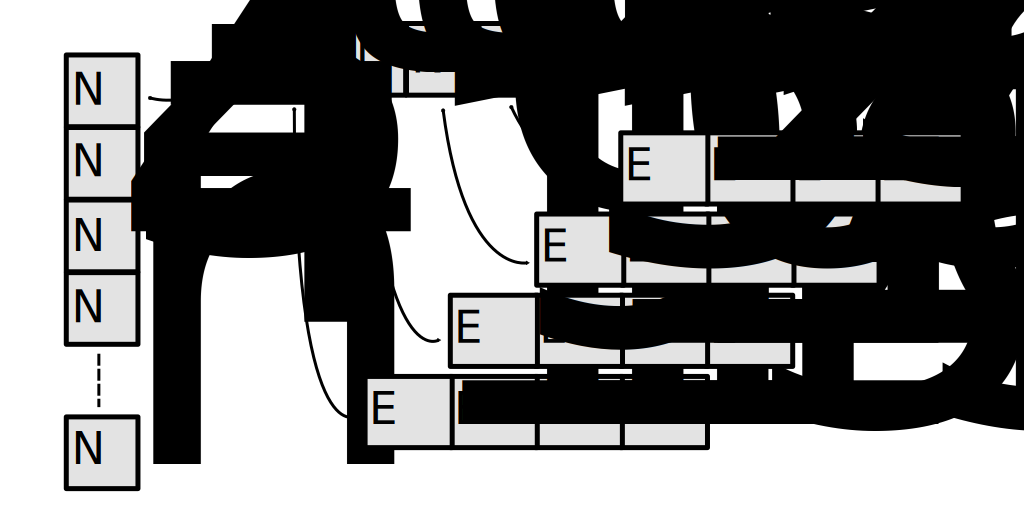
\includegraphics[scale=0.35]{networkx-dict}
		\caption[Rappresentazione nodi e archi networkx]{Rappresentazione grafica dei nodi e degli archi descritti in networkx.}
		\label{fig:networkx-dict}
	\end{centering}
\end{wrapfigure}

Questa scelta, oltre a rappresentare il modo più corretto per
implementare tale struttura\cite{python-graph}, permette un rapido
accesso ai nodi e agli archi che li mettono in relazione.

Oltre a specificare un identificativo univoco da assegnare a nodi e archi,
è possibile definire delle proprietà che possono essere dei tipi primitivi
o degli oggetti.

\subsection{Tipi di grafo}
Vi sono quattro differenti tipologie di grafo a disposizione:
\begin{itemize}
	\item grafo non diretto,
	\item grafo diretto,
	\item multigrafo non diretto,
	\item multigrafo diretto
\end{itemize}
Nel grafo non diretto, all'aggiunta di un arco $(u, v)$ tra
i nodi $u$ e $v$ viene aggiunto automaticamente un
arco $(v, u)$.

I multigrafi permettono di definire molteplici archi delimitati dalla
stessa coppia di nodi. In tal caso la definizione dell'identificativo
di un arco è di maggiore importanza, visto che sarà necessario
discriminare l'arco desiderato da un insieme di collegamenti
tra la stessa coppia di nodi. Per i multigrafi (diretti e non)
NetworkX permette, all'aggiunta di un arco, di specificare la chiave
(identificativo) associato all'arco che si sta inserendo; nel caso in cui
l'utente non definisce un identificativo, l'oggetto rappresentante il grafo
fornisce automaticamente un numero intero da assegnarli non ancora
utilizzato.

\subsection{Perchè è stata scelta e limiti}
\label{sec:nx-why-limits}
Il contenuto di un file GFA è direttamente rappresentabile mediante
un grafo, per questo sfruttare una libreria già esistente ha permesso
di velocizzare i tempi di sviluppo.

NetworkX offre la miglior implementazione dei grafi scritta in Python,
sfruttando dove richiesto librerie matematiche anche di basso livello
per garantire prestazioni molto alte in termini di velocità. La vasta
gamma di algoritmi a disposizione, uno sviluppo costantemente
attivo\cite{networkx-github} e un'ampia documentazione rendono
questa libreria un'ovvia candidata per lo sviluppo di \pygfa.

Uno svantaggio, dovuto all'implementazione direttamente in Python di
Networkx, è il consumo piuttosto elevato di memoria richiesto
per contenere il grafo. Tale peso è dovuto principalmente
all'uso dei dizionari come struttura di rappresentazione di nodi ed
archi. In \pygfa tale inconveniente è possibile notarlo specialmente
nei dizionari degli archi, che arrivano ad occupare più
di \SI{2}{\kilo\byte}.

Un altro aspetto negativo della libreria è che non permette l'impiego degli
algoritmi considerando le proprietà di archi e nodi. Ciò significa
che, supponendo di avere degli archi colorati (blu, giallo, rosso),
non è possibile applicare gli algoritmi solo agli archi di uno specifico
colore. Per questo in \pygfa si è reso necessario andare a ridefinire
(sfruttando il sorgente) gli algoritmi di interesse andando
a considerare nell'algoritmo i nodi definiti da un iteratore, che li
seleziona in base ad una proprietà dell'arco, evitando
di considerare l'intera lista di adiacenza del singolo nodo.

% Coverage.py
\section{unittest e Coverage.py}
Python è un linguaggio dinamico, per questo ogni
riga di un programma viene analizzata solo nel momento
in cui lo script viene lanciato. Ciò vuole significare che un errore
(esclusi quelli di sintassi) non può essere individuato prima
della sua esecuzione.

Per questo motivo nello sviluppo di \pygfa si è scelto di scrivere
i casi di test con la libreria \emph{unittest}, fornita direttamente
con l'interprete, e successivamente si sono andati ad analizzare
gli script dei casi di test con \emph{Coverage.py}.

Coverage.py è un programma Python in grado di misurare la
copertura del listato scritto, annotando le parti del codice che
sono state eseguite e creando un report (su file o su interfaccia web)
indicando le righe che necessitano ulteriore copertura.

Entrambi gli strumenti sono stati presi in considerazione per via
della loro facilità di integrazione nello sviluppo, per
la loro chiarezza nell'esposizione degli errori e delle statistiche
e per la loro diffusione tra gli sviluppatori.

\subsection{Funzionamento}
Lo strumento di analisi per la copertura prende in input un programma Python il quale
viene eseguito linea per linea. Tutti i file coinvolti nel programma
(poiché contenenti funzioni, classi o variabili usate presenti
nello script) vengono considerati nel calcolo della copertura. La
misura della copertura avviene sia per singolo file che sull'intero
insieme di file coinvolti dal programma. La copertura
sul singolo file viene calcolata come:
\begin{equation}
Cov(f) = \frac{\#linee_{coperte}}{\#linee_{totali}}
\end{equation}

unittest invece permette di confrontare il risultato di un'operazione rispetto
ad un valore atteso, fermando l'esecuzione nel caso in cui uno di questi
confronti fallisce. E' possibile inoltre confrontare il comportamento atteso
da una certa operazione, come l'invocazione di un'eccezione in caso di
operazioni non valide.

% Pylint
\section{Pylint}
\nocite{pylint}
Pylint è uno strumento di analisi del codice, curato dalla
Python Code Quality Authority\cite{pycqa}, in grado di applicare
una serie di regole atte a verificare:
\begin{itemize}
	\item la compatibilità del programma rispetto le convenzioni stabilite
		dal linguaggio\cite{python-pep8};
	\item problemi di importazione delle librerie;
	\item la presenza di variabili usate in un contesto in cui il loro valore
		sarebbe indefinito;
	\item il verificarsi di codice duplicato, sia all'interno dello stesso file
		sia fra sorgenti diverse.
\end{itemize}

Lo strumento quindi non solo fornisce dei meccanismi di standardizzazione
del codice, ma effettua quelle operazioni complementari a unittest e coverage.py
per la verifica della correttezza, da un punto di vista sintattico e simbolico,
del programma.

\subsection{Come è stato usato}

Pylint è uno strumento di \emph{controllo}, che fornisce suggerimenti riguardanti molti
aspetti del codice. Osservare tutti gli avvertimenti e risolvere tutti i problemi
rilevati avrebbe richiesto un prolungamento dei termini di consegna, oltre che
costituire un lavoro non prioritario.
Il suo impiego in \pygfa è voluto per cercare di uniformare una nuova libreria
Python con le convenzioni e le pratiche più comuni che la maggior parte degli
utilizzatori di questo linguaggio si aspettano, fornendo loro un ambiente
familiare nel quale la complessità non sia data dalla costante ricerca nella
documentazione di nomi e comportamenti insoliti circa elementi che compongono
la libreria. Generalmente si sono cercati di risolvere tutti quei problemi relativi gli standard
di nomenclatura oltre che problemi di analisi simbolica che avrebbero compromesso
il corretto funzionamento di \pygfa.

\addcontent{Indicare il numero di issue al momento della consegna di \pygfa.}

\section{Sphinx e Read the Docs}
\label{seq:sphinx-rtd}
Sphinx è uno strumento per la generazione automatizzata di documentazione
del codice. Grazie a questo strumento è possibile ricavare un manuale
ben formatto direttamente dal sorgente, il quale deve essere scritto
secondo un linguaggio ben specifico per indicare elementi di rilievo
del codice, come parametri, valori di ritorno, eccezioni,
note o link.

Sphinx è stato creato creato in origine per la documentazione ufficiale
del linguaggio Python\cite{python-doc} e fin da subito si è sparso
come strumento di aiuto nella documentazione di programmi scritti
non solo in questo linguaggio, ma anche in molti altri linguaggi supportati,
vista la sua flessibilità e i risultati ottimi che produce.

Esso usa il \emph{reStructuredText} come linguaggio di markup, permettendo
un'ampia espressività e una vasta gamma di notazioni come link (interni ed esterni),
definizione di tag personalizzati e liste (ordinate e non) oltre la possibilità
di scrivere formule matematiche in \LaTeX.

Sphinx permette di generare la documentazione finale nei formati più comuni:
HTML (con supporto mobile nativo), PDF e EPUB. Solitamente la scelta
più diffusa (che \pygfa segue) è quella di produrre la documentazione in
HTML e di renderla disponibile su \emph{Read the Docs}.

\phantomsection
\label{seq:sphinx}
Read the Docs è una piattaforma online, supportata dalla community,
appositamente pensata per salvare, catalogare e rendere disponibile
la documentazione scritta con Sphinx.
Il sito fornisce un ambiente Python e permette di collegare la documentazione
direttamente ad un repository di progetto su Github, evitando così di
dover mantenere aggiornate due copie di un singolo progetto separate.
Il sito usa l'ambiente Python per generare la documentazione di
progetto, permettendo di aggiungere le dipendenze del codice mediante
file di testo. La procedura è automatizzata (vedere figura
\ref{fig:rtd-build}) e il codice HTML risultante viene pubblicato sulla
piattaforma al termine del processo.

Grazie a Sphinx e Read the Docs è stato possibile documentare \pygfa
in modo facile e veloce, evitando di costruire soluzioni \emph{ad-hoc}
per la sua distribuzione e manutenzione e, allo tempo stesso,
si è riusciti ad ottenere un risultato più che accettabile utilizzando
i temi predisposti della piattaforma, garantendo all'utilizzatore
una facile consultazione sia da desktop che da mobile, una visione
del sorgente direttamente dalla documentazione e una funzione
di ricerca efficace.

\begin{figure}[h]
	\center
	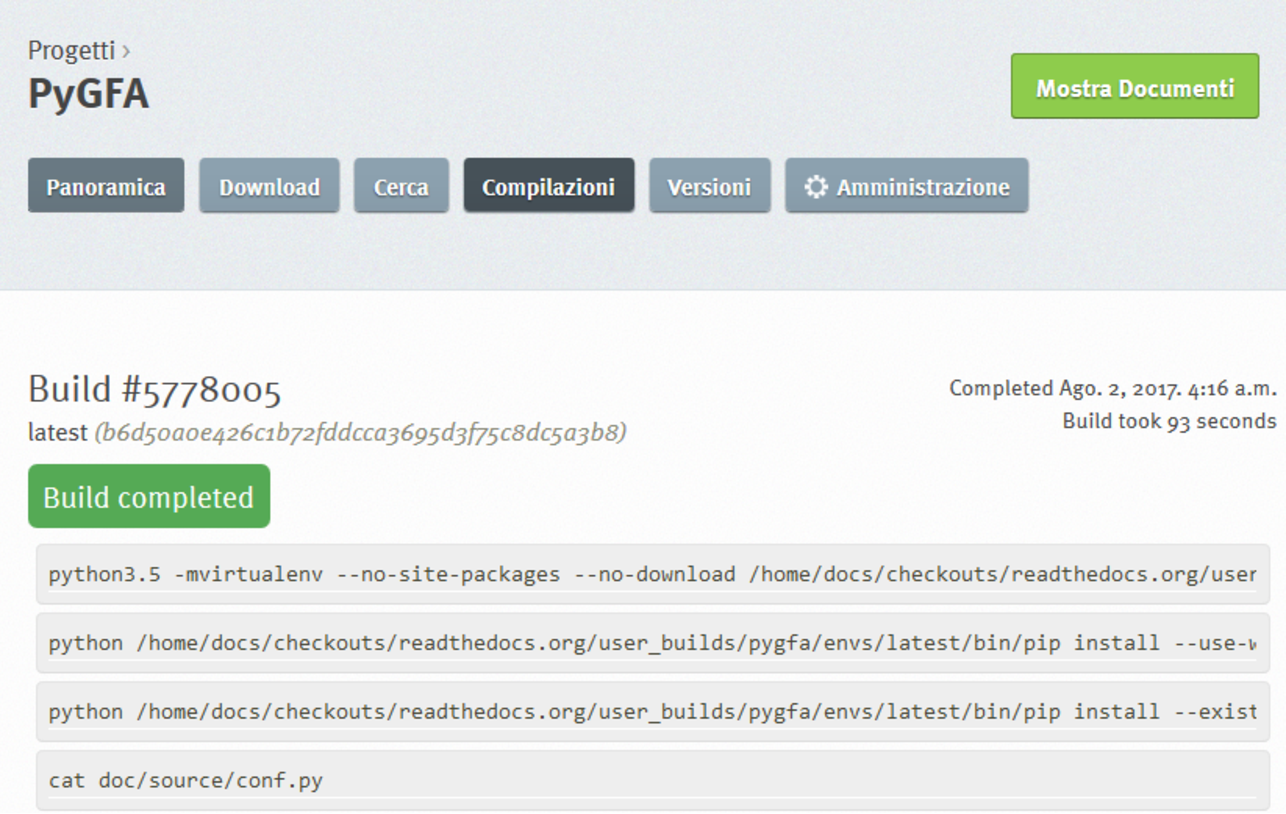
\includegraphics[scale=0.65]{rtd}
	\caption[Schermata di build di Read the Docs.]{Interfaccia per la generazione della documentazione in Read the Docs.}
	\label{fig:rtd-build}
\end{figure}

% git e GitHub
\section{git e GitHub}
\nocite{git}
\emph{git} è un sistema di controllo versione, ideato da Linus Torvalds per
gestire lo sviluppo del kernel Linux, tra i più utilizzati al mondo.
Esso permette di gestire progetti di ogni dimensione, garantendo velocità,
coerenza e ripristino fra le diverse tappe di sviluppo di un progetto.

\begin{wrapfigure} {O} {0.35\textwidth}
	\begin{centering}	
		
\includegraphics[scale=0.5]{git-logo}
		\caption[Logo git]{Logo dello strumento di controllo versione git.}
	\end{centering}
\end{wrapfigure}

Il programma permette, una volta inizializzato all'interno di una cartella,
di gestire i file in base ai cambiamenti ad essi effettuati. Per integrare
un cambiamento apportato ad un file è necessario aggiungerlo a quella
che viene chiama \emph{staging area}, contenente l'insieme
di file modificati a partire dall'ultimo stato aggiornato del sistema.
Generalmente i file nella staging area sono accomunati da un contesto
comune (una modifica che coinvolge per lo stesso motivo quello specifico
insieme di file), ma ai fini del sistema ciò non è un requisito indispensabile.
Terminate le modifiche e aggiunte alla staging area è necessario integrare
tali modifiche nel sistema mediante una \emph{commit}, un'operazione
che crea un identificativo univoco dello stato del sistema nel momento esatto
in cui i cambiamenti vengono integrati con esso. Grazie alla creazione
di questo identificativo è possibile ritornare nell'esatto stato
del sistema indicato, nel caso fosse necessario.

Git permette non solo di lavorare ad un progetto procedendo in un'unica
sequenza di sviluppo, ma permette la creazione di più diramazioni parallele
(\emph{branch}), indipendenti dalle future modifiche apportate al sistema,
che possono procedere nello sviluppo. Tali diramazioni garantiscono un
ambiente di lavoro isolato e stabile nel quale un singolo sviluppatore può
concentrare il suo sviluppo, senza preoccuparsi delle modifiche che altri
sviluppatori potrebbero apportare al sistema, per poi far ricongiungere
il componente nella principale sequenza di sviluppo (solitamente indicato
dal branch \emph{master}).

La flessibilità di sviluppo che questo strumento offre permette di strutturare
al meglio le diverse fasi di implementazione di un progetto, in piena coerenza con
un processo agile o di extreme programming. In \pygfa tale caratteristica
si è rivelata di fondamentale importanza, permettendo di suddividere
fasi di refactoring o di ridefinizione della struttura di progetto (operazioni
molto delicate da un punto di vista della stabilità della libreria) in un
ambiente controllato e reversibile in caso di problemi.

Completate le modifiche ed effettuata la commit, è possibile sincronizzare
i cambiamenti locali con una repository remota, un luogo decentralizzato
sul quale il lavoro viene salvato e grazie al quale è possibile condividere
il progetto con i propri collaboratori. Una tra le più famose piattaforme
che permettono di ospitare un repository git remoto è \emph{GitHub}.

GitHub è un sito che offre funzionalità paragonabili a quelle che Read
the Docs (vedi sezione \ref{seq:sphinx-rtd} a pagina \pageref{seq:sphinx})
fornisce per Sphinx. Permette di ospitare repository remote, catalogarle
per una maggiore accessibilità (se pubbliche) offrendo un'interfaccia
intuitiva per:
\begin{itemize}
	\item la creazione di \emph{tag} per il rilascio delle versioni stabili del sistema,
	\item la creazione di aree di discussione relative a bachi, miglioramenti e problematiche
		generali, fornendo agli sviluppatori un luogo centralizzato e coerente
		per la discussione di queste tematiche,
	\item lla creazione di punti di branching e analisi delle diverse ramificazioni del sistema
		e dell'attuale sequenza di sviluppo del progetto,
	\item la navigazione dell'intero progetto, con la possibilità di ispezionarlo
		ricreandone lo stato dopo una specifica commit,
	\item la visione di statistiche relative le commit effettuate da chiunque
		abbia contribuito al sistema, con la possibilità di analizzare le modifiche
		apportate a livello di singola commit.
\end{itemize}

Il ruolo che questi due strumenti hanno avuto e avranno nello lo sviluppo
di \pygfa è \emph{incalcolabile}. Non solo ai fini del salvataggio del
progetto, della sua gestione e della sua reperibilità, ma anche per la
possibilità che esso offre di permettere ad un qualsiasi sviluppatore di
effettuare facilmente una diramazione del codice ai fini di poterlo
riscrivere in base alle proprie necessità, senza doversi cimentare
nello sviluppo di un sistema nuovo (\emph{fork}).

% Bandage
\section{Bandage}
\label{sec:bandage}
\nocite{doi:10.1093/bioinformatics/btv383}
Bandage è un programma per la visualizzazione grafica di grafi
di assemblaggio. Questo strumento è in grado di visualizzare
grafi descritti da file GFA1, per questo il suo impiego
è stato di vitale importanza nell'analisi dei collegamenti presenti fra
le sequenze, specialmente nei casi di dovetail overlap, che descrivono
un continuum nel genoma e che per tanto costituiscono un'informazione
di rilievo per una libreria che si occupa della gestione di questi file.

\section{Conclusioni}
In questo capitolo sono stati presentati gli strumenti impiegati nello sviluppo
di \pygfa, nella fase di test e di documentazione indicando i dettagli
che si sono rivelati di particolare importanza ai fini implementativi del sistema.

% GFA specifications
\chapter{Le specifiche GFA}

In questo capitolo verrà fornita un'ampia panoramica sulle specifiche
GFA, sulle linee presenti e sulle diverse circostanze di assemblaggio
di sequenze che possono essere rappresentate.
Verrà inoltre fornita una breve introduzione ad alcuni concetti
biologici riguardanti gli elementi che compongono DNA e RNA e
la loro struttura, necessarie a comprendere le diverse situazioni
descritte nelle specifiche.

\section{Introduzione a GFA, motivazioni e struttura}
GFA è l'acronimo per Graph Assembly Format, è un
formato per la rappresentazione dei legami presenti fra le sequenze di
un genoma al fine di riuscire a ricostruirne la struttura.
Le motivazioni che risiedono alla base della proposta per un nuovo
formato consistono nell'uniformare le notazioni che programmi
di visualizzazione, di assemblaggio e di manipolazione potessero
utilizzare.

La prima versione della specifica GFA viene indicata col termine
GFA1. Questa prima versione, come vedremo successivamente,
limita la descrizione delle possibili situazioni in cui due sequenze
possono trovarsi in relazione. Per questo motivo, e per estendere
maggiormente l'insieme delle informazioni utili da descrivere,
è stata sviluppata una seconda specifica, indicata con GFA2.
Questa specifica generalizza, usando un'unica notazione,
i collegamenti fra sequenze descritti da GFA1 e permette inoltre
di descrivere relazioni di ogni tipo fra due sequenze.
GFA2 è un \emph{superset} di GFA1 e come tale permette
(con un minimo numero di operazioni) di trasformare un file GFA2
nell'analogo (rappresentabile) in GFA1. Questa seconda specifica
è stata appositamente pensata per permettere la descrizione di
sequenze e collegamenti imponendo un minimo numero di vincoli,
permettendo all'utilizzatore di impiegarla per la descrizione di dati
indipendentemente dai dettagli che questi forniscono.

Entrambe le specifiche adoperano la stessa formattazione delle linee.
Una linea descrive un'informazione di assemblaggio, sia
essa una sequenza, un collegamento o un insieme di elementi.
In ogni riga, il primo carattere indica
l'identità della linea stessa alla quale seguono, separati esclusivamente
da tabulazioni, gli elementi che costituiscono l'informazione
che la linea descrive e che prendono il nome di \emph{campi}.
I campi possono essere definiti o meno, nel qual caso l'assenza
dell'informazione viene indicata con un asterisco \texttt{*}.

In ogni linea di entrambe le specifiche è possibile descrivere campi
opzionali (che possono essere predefiniti per una linea o introdotti
direttamente dall'utente), descritti nel formato \texttt{TAG:TIPO:CONTENUTO}
dove \texttt{TAG} è una sequenza di due caratteri alfanumerici
(in maiuscolo se il campo è predefinito dalla linea, in minuscolo
altrimenti) che identifica l'informazione che esso indica.
Il \texttt{TIPO} di un campo viene anch'esso descritto da un
identificatore, ciascuno indicante il seguente contenuto:

\noindent
\begin{table}[h]
	\rowcolors{1}{white}{lightgray}
	\begin{tabularx}{\textwidth}{ | X | l | }
		\hline
		Tipo	&	Descrizione\\
		A 		&	Singolo carattere stampabile(escluso lo spazio)\\
		i 		&	Intero con segno\\
		f 		&	Decimale con precisione singola\\
		Z		&	Stringa stampabile (incluso lo spazio)\\
		J		&	Stringa JSON, escludendo caratteri di newline e di tabulazione\\
		H 		&	Array di Byte in formato esadecimale\\
		B 		&	Array di interi o di decimali\\
		\hline
	\end{tabularx}
	\caption{Tabella dei tipi che è possibile usare per specificare campi opzionali.}
	\label{tab:optfield-type}
\end{table}

\begin{wrapfigure} {O} {0.65\textwidth}
        \begin{centering}
                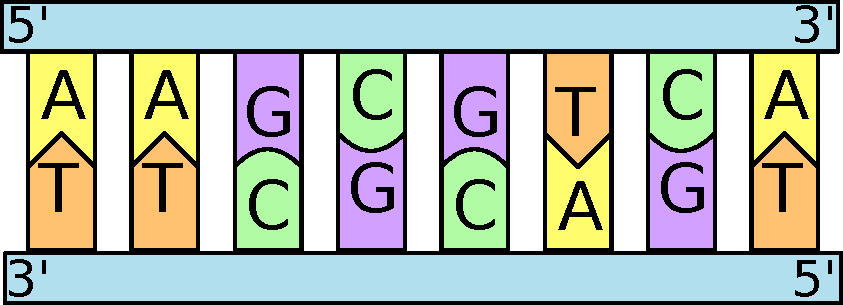
\includegraphics[scale=0.5]{dna-strand}
                \caption[Rappresentazione del DNA]{Rappresentazione grafica degli strand che compongono il DNA.}
                \label{fig:dna-strand}
        \end{centering}
\end{wrapfigure}

Mentre verranno analizzate le linee delle due specifiche, è essenziale
avere un'idea di cosa sia una sequenza e di come questa può essere in
relazione con le altre.
Con il termine sequenza viene indicata una \emph{sequenza nucleotidica},
un susseguirsi di lettere che denotano le unità molecolari che compongono
gli acidi nucleici di RNA e DNA (\emph{nucleotide}).
Una sequenza è priva di un ordine specifico, ma è possibile attribuirgliene
uno osservando la composizione del tipo di legame che collegano
gli elementi costitutivi il nucleotide, in base all'orientamento del
legame presente tra le unità di carbonio 3' di un un'unità
e la stessa unità 5' della successiva. Grazie a tale osservazione
è possibile individuare un ordinamento che verrà definito
come 5'3'.

Oltre questa considerazione, bisogna tenere conto che
l'informazione presente nel DNA
è la stessa a parità di estremità, ma in ordine inverso e
complementato (vedi figura \ref{fig:dna-strand}) (sostituendo
la citosina con la guanina e
l'adenina con la timina). Nel caso di RNA alla timina
si sostituisce l'uracile, ma il processo di formazione del RNA
prevede anch'esso questa operazione di complementazione
della sequenza.

Ergo, quando si considera una sequenza (nel caso
dell'assemblaggio del DNA), è necessario tenere presente
che un collegamento fra due sequenze potrebbe considerare
una sequenza posta sullo strand (una delle estremità
che compone l'elica del DNA) opposto e di conseguenza una loro
sovrapposizione potrebbe richiedere un preprocessamento della
stringa che la porti ad essere coerente con l'altra, operazione
che prende il nome di \emph{reverse and complement}.

% GFA1
\section{Linee GFA1}
GFA1 è la prima versione della specifica, essa si concentra nella descrizione
delle sequenze, collegate tra loro da una relazione di \emph{contenimento}
o di \emph{successione}.

Le linee previste dalla specifica sono header, segment, link, containment
e path.

L'header è una riga il cui scopo è quello di indicare la versione della specifica
in uso, può ripresentarsi più volte all'interno del file per indicare parametri
opzionali validi per tutti gli elementi. Tale linea viene indicata con il simbolo \texttt{H}.

\subsection{Segment}
La linea di Segment (indicata con il simbolo \texttt{S}) descrive in termini
generici una sequenza, la quale può essere definita o no. All'informazione
viene attribuito un identificativo che deve essere unico in tutto in file.
A queste proprietà se ne possono aggiungere altre, descritte da campi
opzionali, tra i quali la lunghezza (\texttt{LN}) e
il conto dei \emph{k-meri} (l'insieme di tutte le possibili sottostringhe
di lunghezza k contenute nella stringa).

\begin{lstlisting}[basicstyle=\ttfamily, caption=Una possibile Segment line.]
S	5	CCCGGGGTAA		LN:i:10
\end{lstlisting}

\subsection{Link}
\label{sec:link}
I Link (indicati dal simbolo \texttt{L}) sono il principale
tipo di relazione fra due sequenze. Essi
indicano una sovrapposizione fra le sequenze indicate da due Segment.
Nello specifico, un Link fra due Segment indica che la parte terminale
della prima sequenza è coinvolta in una sovrapposizione (\emph{overlap})
con l'inizio della seconda; il termine che descrive esattamente questa situazione
è \emph{dovetail overlap} tradotta in sovrapposizione a coda di rondine.
Tale tipologia di collegamento costituisce
un'informazione di rilievo nell'analisi dell'assemblaggio poiché descrive
un susseguirsi fra due sequenze.

Il link non solo descrive questa situazione, ma indica anche quale
estremità della sequenza è coinvolta nel overlap. Ricordando che
l'informazione contenuta nella struttura elicoidale del DNA è la stessa a parità
di estremi (ma in senso inverso e complementata), è possibile
che due sequenze siano contigue (in una situazione di dovetail
overlap) considerando la loro provenienza da due estremità
diverse dell'elica (strand).
Il link permette di esprimere il collegamento considerando anche questa
particolarità; per farlo esso utilizza un segno ``\texttt{+}'' per indicare
che la sequenza non necessita di alcun processamento nel suo
coinvolgimento nella sovrapposizione, mentre utilizza un segno ``\texttt{-}''
per esplicare la necessità di effettuare un' operazione di reverse
and complement sulla sequenza prima di poterla considerare
nel overlap.

Visto che, come si diceva poc'anzi, un Link descrive una sovrapposizione
tra la fine della prima sequenza e l'inizio della seconda (indipendentemente
dai segni associati alle due sequenze coinvolte), ciò da luogo a quattro
possibili situazioni:
\begin{itemize}
	\item la parte destra della prima sequenza si sovrappone con la parte
		sinistra della seconda (vedi figura \ref{fig:dov-ov}\subref{fig:dov-ov++});
	\item la parte destra della prima sequenza si sovrappone con la parte
		destra della seconda (vedi figura \ref{fig:dov-ov}\subref{fig:dov-ov+-});
	\item la parte sinistra della prima sequenza si sovrappone con la parte
		sinistra della seconda (vedi figura \ref{fig:dov-ov}\subref{fig:dov-ov-+});
	\item la parte sinistra della prima sequenza si sovrappone con la parte
		destra della seconda (vedi figura \ref{fig:dov-ov}\subref{fig:dov-ov--}).
\end{itemize}

\captionsetup{justification=centering}
\begin{figure}[h]
	\begin{subfigure}{.5\linewidth}
	  \centering
	  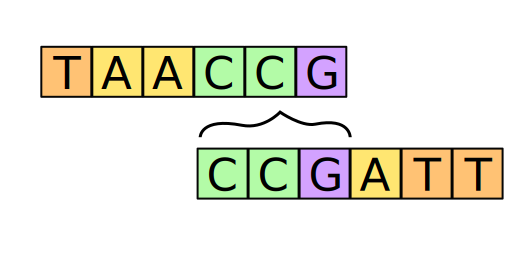
\includegraphics[scale=0.4]{dov_ov_++}
	  \caption{}
	  \label{fig:dov-ov++}
	\end{subfigure}%
	\begin{subfigure}{.5\linewidth}
	  \centering
	  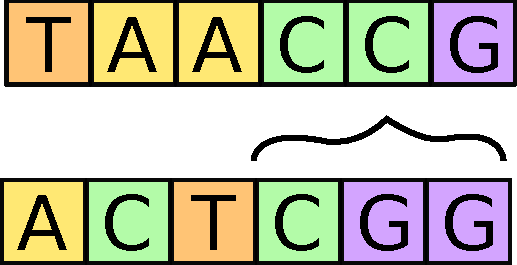
\includegraphics[scale=0.4]{dov_ov_+-}
	  \caption{}
	  \label{fig:dov-ov+-}
	\end{subfigure}%
	
	\bigskip%
	
	\begin{subfigure}{0.5\linewidth}
	  \centering
	  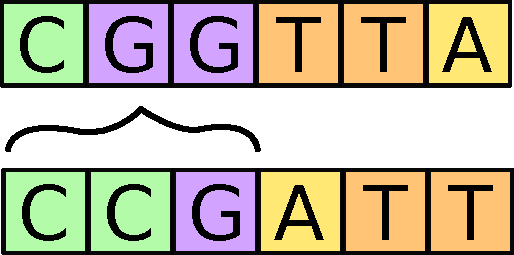
\includegraphics[scale=0.4]{dov_ov_-+}
	  \caption{}
	  \label{fig:dov-ov-+}
	\end{subfigure}%
	\begin{subfigure}{0.5\linewidth}
	  \centering
	  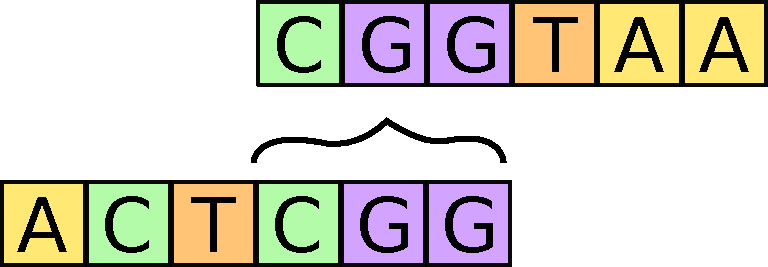
\includegraphics[scale=0.4]{dov_ov_--}
	  \caption{}
	  \label{fig:dov-ov--}
	\end{subfigure}
	
	\captionsetup{justification=justified}
	\caption[Rappresentazione delle possibili situazioni di dovetail overlap]{
		\textit{(a)} Dovetail overlap senza bisogno di alterare le sequenze.
		\textit{(b)}  Dovetail overlap dove la seconda sequenza necessita
	  		di un'operazione di reverse and complement per sovrapporsi alla prima.
	  	\textit{(c)} Un'operazione di reverse and complement deve essere eseguita
	  		sulla prima sequenza, affinché ci sia un overlap.
	  	\textit{(d)} Entrambe le sequenze richiedono operazioni di reverse and complement.}
	\label{fig:dov-ov}
\end{figure}
\captionsetup{justification=justified}

Oltre a questa considerazione sulle sequenze, il Link fornisce una descrizione
dell'allineamento, dato da una stringa CIGAR. Una stringa CIGAR è
una serie di lettere e numeri che descrivono lo stato di somiglianza
fra le due sequenze.
Tra i campi opzionali che il Link predispone si trova il campo
\texttt{ID}, mediante il quale è possibile riferirsi a tale
linea.
\clearpage

\subsection{Containment}
\label{sec:containment}
\begin{wrapfigure} {O} {0.35\textwidth}
	\begin{centering}	
		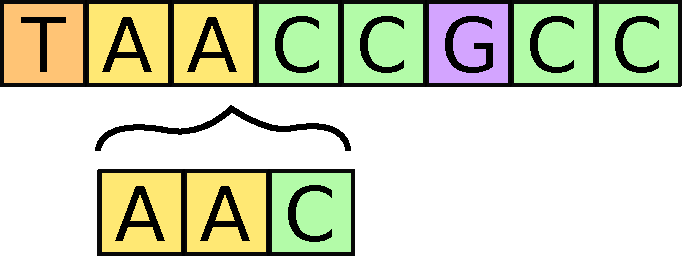
\includegraphics[scale=0.35]{containment}
		\caption[Rappresentazione di una situazione di contenimento fra sequenze]
		{Una rappresentazione grafica della situazione di contenimento fra due sequenze.}
		\label{fig:containment}
	\end{centering}
\end{wrapfigure}
Le linee di Containment (indicate con il simbolo \texttt{C})
descrivono sovrapposizioni fra sequenze nelle quali una stringa intera
è contenuta nell'altra.
I campi descrivono le stesse informazioni dei Link, ma è bene notare
i dettagli circa le posizioni delle sequenze che una sovrapposizione di
questo tipo comporta.
Date due sequenze $s1$ ed $s2$, un Containment tra la sequenza $s1$ e la
sequenza $s2$ indica che la sequenza $s1$ \emph{contiene} la sequenza
$s2$. In tale situazione vuole significare che la sovrapposizione comincia
dal primo carattere della sequenza di $s2$ e continua fino all'ultimo
(vedi figura \ref{fig:containment}).

Oltre ai classici campi che descrivono i nodi indicanti le sequenze coinvolte,
il loro orientamento nella sovrapposizione e l'allineamento; queste linee hanno un campo
che indica la posizione di inizio della sequenza contenuta nella sequenza
contenitrice.

\subsection{Path}
Un Path (indicato dal simbolo \texttt{P}) descrive un susseguirsi di
sequenze collegate esclusivamente da Link. Indica pertanto un percorso
di sequenze contigue all'interno del grafo. Queste linee
indicano esclusivamente gli identificativi e l'orientamento delle sequenze
coinvolte nel percorso cui seguono l'insieme delle stringhe CIGAR relative
l'allineamento delle sequenze prese a due a due.

\newpage
\captionsetup{justification=centering, singlelinecheck=false}
\begin{lstlisting}[basicstyle=\ttfamily, frame=topline, caption=Un esempio di file GFA 1.]
H	VN:Z:1.0
S	11	ACCTT
S	12	TCAAGG
S	13	CTTGATT
L	11	+	12	-	4M
L	12	-	13	+	5M
L	11	+	13	+	3M
P	14	11+,12-,13+	4M,5M
\end{lstlisting}
\captionsetup{justification=justified, singlelinecheck=false}


\section{GFA2}
GFA2 come accennato in precedenza è un'estensione di GFA1, pensata
per fornire più libertà all'utente circa le informazioni che è possibile descrivere.
Le linee appartenenti a questa specifica non comprendono campi opzionali
predefiniti, l'utente è libero di definire i campi aggiuntivi che più ritiene opportuni
per la sua applicazione.


\subsection{Segment}
Queste linee sono analoghe ai Segment in GFA1, ai campi viene aggiunto
un numero intero per descrivere la lunghezza della sequenza.
La lunghezza non vuole essere l'esatta lunghezza della sequenza, ma
vuole indicare la grandezza che tale sequenza assume quando rappresentata
da un programma di disegno (come Bandage, descritto a pagina \pageref{sec:bandage}).
Nell'indicare le sequenze non viene più richiesto l'uso di caratteri IUPAC\cite{wiki:acid-notation},
la sequenza può essere descritta con un qualsiasi carattere stampabile,
nello specifico dal simbolo ``\texttt{!}'' al simbolo ``\texttt{\textasciitilde}''
della tabella ASCII.

\subsection{Edge}
\begin{wrapfigure} {O} {0.35\textwidth}
	\begin{centering}	
		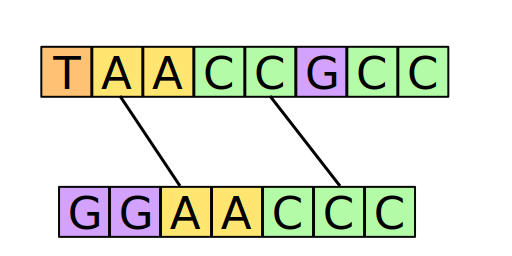
\includegraphics[scale=0.35]{generic-overlap}
		\caption[Rappresentazione di una situazione generica di sovrapposizione fra sequenze]
		{Una rappresentazione grafica di una generica sovrapposizione fra sequenze.}
		\label{fig:generic-overlap}
	\end{centering}
\end{wrapfigure}
La linea di Edge (indicata con la lettera \texttt{E}), indica un qualsiasi
tipo di sovrapposizione. Essa quindi generalizza le linee di Link e Containment
ed aggiunge la situazione in cui una generica parte di una sequenza
è sovrapposta ad una qualsiasi parte (non solo agli estremi) di
un'altra (come rappresentato in figura \ref{fig:generic-overlap}).

Questa linea, come Link e Containment, fornisce gli identificatori
delle sequenze coinvolte nel overlap e i rispettivi orientamenti, cui
si aggiungono le \emph{posizioni} di inizio e fine delle parti
delle rispettive sequenze sulle quali si svolge la sovrapposizione.
La posizione è un intero che parte da 0 (descrivendo il primo
carattere della sequenza) e termina in posizione pari alla
lunghezza stessa della sequenza, all'ultima posizione della sequenza
si pone il simbolo ``\texttt{\$}'', non farlo costituirebbe un errore.

In questo modo si avrà che una situazione di dovetail overlap
verrà indicata da un edge in cui le posizioni delle due sequenze
sono  $inizio1=0$ e $fine2=y\$$ o $fine1=x\$$ e $inizio2=0$;
mentre una situazione di contenimento viene descritta
da un edge in cui le posizioni delle sequenze sono $inizio1=0$ e 
$fine1=x\$$ o $inizio2=0$ e $fine2=y\$$. Si osservi che mentre
un contenimento in GFA2 non impone alcun ordine circa la sequenza
contenuta e quella contenitrice, un Containment in GFA1 prevede
che la prima sequenza sia la contenitrice e la seconda sia la contenuta;
inoltre in GFA2 non vi è alcun campo obbligatorio che indica l'inizio della
sequenza contenuta, diversamente da GFA1.

Come in GFA1 è possibile specificare l'allineamento, non solo mediante
stringa CIGAR, ma indicando una traccia DAZZLER (un indicatore
per eseguire l'allineamento fra sequenze in un tempo quasi lineare).
Quindi non solo GFA2 permette di descrivere la natura dell'allineamento tramite
CIGAR string, ma anche di descrivere un modo veloce per calcolarlo usando
le tracce DAZZLER. Come nelle altre situazioni delle specifiche, in caso
di mancata informazione viene posto un asterisco in tale campo.

Questa generalizzazione delle possibili sovrapposizioni tra due sequenze
permette di usare la specifica non solo per la descrizione di grafi di assemblaggio,
come nel caso di GFA1; ma anche di rappresentare, in un unico formato,
i risultati provenienti da diversi stadi del processo di assemblaggio.

\subsection{Fragment}
Le linee di Fragment (indicate con la lettera \texttt{F}) indicano un
collegamento fra una sequenza indicata nel file e una sequenza presente in un file esterno.
Il collegamento esprime un allineamento fra le due sequenze, in modo analogo ad
un Edge.

\subsection{Gap}
Le linee di Gap (indicate con la lettera \texttt{G}) indicano uno spazio
presente fra due sequenze, indicando la distanza che le separa e la
varianza di tale supposizione.

\subsection{Group}
I gruppi in GFA possono essere di due tipi, gli OGroup (indicati con la lettera \texttt{O})
e gli UGroup (indicati con la lettera \texttt{U}). I primi indicano una sequenza ordinata di elementi
GFA2 (escludendo gli UGroup) che individuano un percorso all'interno del grafo, mentre
gli UGroup indicano un insieme di elementi del grafo privi di ordine. Entrambi
i gruppi descrivono un sottografo che è possibile ricavare
dal grafo descritto dal file GFA.

\captionsetup{justification=centering, singlelinecheck=false}
\begin{lstlisting}[basicstyle=\ttfamily\scriptsize, frame=topline, caption=Un esempio di file GFA 2.]
S	1	122	*
S	3	29	TGCTAGCTGACTGTCGATGCTGTGTG
E	1_to_2	1+	2+	110	122$	0	12	12M
S	5	130	*
S	13	150	*
O	14	11+ 12+
S	11	140	*	xx:i:11
F	1	read1+	0	42	12	55	*	id:Z:read1_in_1
U	16	1 3 1_to_3
U	16sub	5 16
S	12	150	*
E	1_to_3	1+	3+	112	122$	0	12	10M
G	1_to_11	1+	11-	120	*
E	11_to_13	11+	13+	20	140$	0	120	120M
\end{lstlisting}
\captionsetup{justification=justified, singlelinecheck=false}

\section{Conclusioni}
In questo capitolo sono state esaminate le due versioni che costituiscono
la specifica GFA, indicando lo scopo del quale ciascuna versione intende
occuparsi e descrivendo i concetti che ciascuna linea vuole rappresentare
nel contesto dell'assemblaggio del genoma. Nel prossimo
capitolo si procederà nella descrizione del lavoro svolto nello sviluppo
di \pygfa \  e di come si è dovuto procedere nella rappresentazione delle
informazioni descritte nelle specifiche.

\printbibliography

\listoftodos[TODO]

\end{document}